%
\documentclass[12pt]{article}
\usepackage{amssymb}
\usepackage{amsmath}
\usepackage{graphicx}
\usepackage{epstopdf}
\usepackage{pdflscape}
\usepackage{tabularx}
\usepackage{longtable}
\usepackage{array}
\usepackage{dsfont}
\usepackage{float}
\usepackage{booktabs}
\usepackage{marvosym}
\usepackage{multirow}
\usepackage{pdflscape}
\usepackage[hyphenbreaks]{breakurl}
\usepackage[hyphens]{url}
\usepackage{setspace}
\usepackage{epigraph}
\usepackage{bm}
\usepackage{textcomp}
\usepackage{bbm}
\usepackage{verbatim}
\usepackage{subcaption}
\usepackage[format=hang,font={small,bf}]{caption}
\usepackage[shortlabels]{enumitem}
\usepackage{graphicx}
\usepackage{natbib,hyperref}
\setlength{\epigraphrule}{0pt}
\setlength\parindent{1cm}
\renewcommand{\baselinestretch}{1}
\renewcommand*{\arraystretch}{1.2}

\setcounter{MaxMatrixCols}{10}

\newcolumntype{L}[1]{>{\raggedright\let\newline\\\arraybackslash\hspace{0pt}}m{#1}}
\newcolumntype{C}[1]{>{\centering\let\newline\\\arraybackslash\hspace{0pt}}m{#1}}

\newcommand{\E}{\mathrm{E}}
\newcommand{\BLP}{\mathrm{BLP}}
\newcommand{\Var}{\mathrm{Var}}
\newcommand{\Cov}{\mathrm{Cov}}
\newcommand{\Corr}{\mathrm{Corr}}
\newcommand{\Prob}{\mathrm{P}}
\newcommand{\N}{\text{N}}

\topmargin=-1.5cm \textheight=23cm \oddsidemargin=-0.0cm
\evensidemargin=-0.0cm \textwidth=16.5cm
\newtheorem{ass}{Assumption}
\newtheorem{definit}{Definition}
\newtheorem{prop}{Proposition}
\newtheorem{thm}{Theorem}
\newtheorem{lem}{Lemma}
\newtheorem{conj}{Conjecture}
\newtheorem{cor}{Corollary}
\newtheorem{rem}{Remark}
\renewcommand{\thesubsection}{\arabic{section}.\arabic{subsection}}
\renewcommand{\thesubsubsection}{\arabic{section}.\arabic{subsection}.\arabic{subsubsection}}

\newcommand\independent{\protect\mathpalette{\protect\independenT}{\perp}}
\def\independenT#1#2{\mathrel{\rlap{$#1#2$}\mkern2mu{#1#2}}}

%Figure path
\def \figroot{stata/out/}
\def \tabroot{stata/out/}

\usepackage{epsfig,hyperref}

\hypersetup{
	pdftitle={ECMA31330 Final Project},    % title
	pdfauthor={Bronckers.Song.Zhang},     % author/Users/veronica/Documents/
	pdfnewwindow=true,      % links in new window
	colorlinks=true,       % false: boxed links; true: colored links
	linkcolor=blue,          % color of internal links
	citecolor=red,        % color of links to bibliography
	filecolor=black,      % color of file links
	urlcolor=blue           % color of external links
}

\allowdisplaybreaks


\begin{document}
\begin{titlepage}
    \begin{center}
        \vspace*{1cm}
        \LARGE
        \textbf{PAPER TITLE Blah Blah\\ Estimating Reaction to Welfare\\ Using Causal Forests\\}
        \vspace{0.5cm}
        \Large
        ECMA 31330 Final Project \\ 
        \vspace{0.8cm}
        \large
        Spring 2021
        \vfill
        \vspace{5cm}
        \textbf{Max Bronckers \\ Veronica Song \\ Dustin Zhang}
    \end{center}
\end{titlepage}


\section{Introduction} 
There has been an increasing adoption of Machine Learning (ML) methods in
economics for algorithmic approaches to causal inference. Whereas initially the
ML methods were avoided due to uncertainty in its consistency, normality, and
efficiency, major developments in methodology has allowed a stable large-sample
confidence interval to be constructed around treatment effect estimates
conditional on multiple covariates.\cite{athey2019ML} \\

One such method is the Bayesian Additive Regression Trees (BART) used by Green and Kern (2012), which
allows heterogeneous treatment effects to be modeled flexibly. Using a Markov
Chain Monte Carlo (MCMC) algorithm that derives effects from the posterior mean
and interval instead of pre-specified tree parameters, BART has a much smoother
and adaptive structure than traditional OLS or single tree models popular in
economics, and is also resilient to problems with
overfitting.\cite{greenkern2012} However, despite its excellent predictive
capacity, BART lacks an asymptotic explanation of the estimates and are thus
difficult for causal inference and application. Though recent work by Ročková
and Saha (2018) suggests modifications to BART that may allow asypmtotic concentration of
the posterior mean around the true mean, the construction of an asymptotic
theory of BART estimates is still an ongoing effort.\cite{rockova2018theory}.
Another such method is the causal forests proposed by Wager and Athey (2017),
which estimates are asymptotically gaussian and unbiased to allow proper
confidence intervals to be constructed around the treatment effect. The
construction of adequate confidence intervals is especially relevant in policy
applications, as consistent estimates can be produced for the treatment
group.\cite{atheywager2019} \\ 

In this paper, we compare the aforementioned two popular ML tools in
heterogenous treatment effects estimation among survey responders using an
empirical dataset. Specifically, we aim to compare uses of BART versus Causal
Forests, using OLS estimates of heterogeneous treatment effects as a benchmark.
To measure the stigma around the word "welfare", we take a survey data of
individual perception on public spending and find the impact of the question
phrasing on the responses. In order to uncover the heterogenous effects of the
question phrasing based on a suite of socioeconomic backgrounds of the
respondent, Green and Kern utilizes BART. Given the theoretical shortcomings of
BART, we aim to make causal forest estimates and compare it to the authors'
findings. The first section of this paper fits a causal forest model on the welfare data and compares our estimates against BART estimates of conditional average treatment effect (CATE) obtained by Green and Kern. However, since in the empirical data we are unable to distinguish the ground truth, we are confined to comparison using interval length and RMSE. In the second section, we examine the causal forest approach under different parameters of a synthetic DGP. Here, taking our DGP as ground truth, we aim to assess conditions under which the causal forest performs well or poorly and check whether these conditions hold in our empirical dataset. \\ 

\section{Causal Forest Estimates of CATE in Welfare Dataset}

\subsection{Discussion of data and motivation for research} 
In our analysis below, we use a survey experiment from GSS which is also utilized by Green and Kern to investigate interactions between treatment and covariates that may lead to treatment effect heterogeneity. The experiment was conducted in the mid-1980s by GSS to study the negative sentiment Americans carry toward government programs labeled as "welfare". Due to associations with racial connotations and poorly managed welfare programs, respondents were found much more likely to endorse government spending for "the poor" than for public "welfare".\cite{rasinski1989}\\

Using BART, Green and Kern illustrates the extent to which such reaction to the question wording as "welfare" varies based on the respondents' background characteristics such as years of education, race, or political alignment. BART has been a popular choice for heterogeneous treatment effect modeling, as its estimates require little parameter tuning, allow accurate detection of interactions between covariates, and are much smoother than those of single tree models. Each individual tree in the forest has only a small effect on the model, by assuming a prior distribution over the tree parameters.\cite{Chipman2010} Such lack of any individual influential trees allow regular model fit of the BART set up. Then, a MCMC algorithm is used to sample tree parameters iteratively from the posterior distribution as the model is fit. Though this assumption of prior distribution and back-fitting algorithm allows BART to be relatively invariant across, in the presence of confounding variables and treatment effect heterogeneity, such regularization may severely bias the treatment effect estimates.\cite{CarvalhoHahnMurray} Moreover, BART estimates still lack theoretical explanation on its asymptotic concentration, making the construction of adequate confidence intervals challenging. 

\subsection{Causal forests and model assumptions} 
For these reasons, we choose to investigate causal forests to estimate the the treatment effect of question wording on welfare program support. Just like BART, causal forests is fit to model non-linear relationships and interactions between covariates. One advantage that causal forests carry over BART is that under weak assumptions, the estimate are asymptotically standard normal distributed with Gaussian confidence intervals.\cite{atheywager2019}. Put in context of economic policy, the presence of an asymptotic theory allows hypothesis testing regarding treatment results and thus aids policy decisions to be made. \\

Causal forests are a specific form of generalized random forests (GRF), which uses adaptive sample splitting criterion taking into account the MSE. To avoid overfitting and reduce bias in the estimates, we also ensure that the tree is 'honest' - the subsample with which we grow a tree is disparate from the subsample with which we drop down and obtain predictions. In our model, we use 80\% of the welfare data to build our tree and estimate treatment effects on the rest with a 5-fold CV for parameters of the model. \\ 

\subsection{Results of analysis and explanation}
We first investigate the average treatment effects (ATE) without conditioning on any covariates for possible effect heterogeneity. We obtain an ATE of 0.336, with a standard deviation of 0.049 and a 95\% confidence interval of (0.256, 0.416). Green and Kern (2012) identified seven variables to condition the treatment effects on: \textit{party identification, political views, age, education, negative attitude towards Blacks}, and \textit{survey year}. Figure 1 displays the CATE estimates obtained by the causal forest model conditional on each of the seven variables. The blue areas represent the 95\% confidence intervals of our estimates. \\

The top two graphs represents CATE as a function of party identification and self-identified political alignment from liberal to conservative. We see around 5 and 3 percentage points difference in the effect of question wording on support for welfare spending between strong Republicans-Democrats and Conservative-Liberals, respectively, controlling for all other covariates. Conservatives and strong Republicans are more likely to be affected by the framing of the survey question as for welfare. The treatment effect conditional on age, on the other hand, is greatest for those in their 30-40s, and diminishes past that age group. The negative bias toward Blacks has a less pronounced moderation on the treatment effect than the BART estimates.  We note that the trends in CATE estimates obtained via causal forest are generally similar to those obtained using BART for most of the covariate groups except education. There seems to be an increasing effect of question wording as the responded receives greater years of education, with the effect peaking at around 11-13 years (with college education). Whereas Green and Kern found no distinct moderation of treatment effects based on education, we find that there is around 5 percentage point difference in treatment effect estimates between those who received no education and those who received post-Graduate education. Lastly, we examine that change in CATE through time (survey year) and find that the treatment effect was strongest during years 1993-1996. Our results once again largely agree with the results obtained through BART, and illustrate that response to "welfare" is highly associated with the respondent's personal background characteristics. \\

We note that our CATE estimates from causal forest are lower than those of BART. This is expected given RIC 




Interpretation of resutls, Comparison to BART (Bias, RMSE, Coverage, Int length) \\








\section{Testing Robustness of Causal Forest Estimates on Multiple DGPs} 

CANNOT GUARANTEE cONFOUNDING IS ADDRESSED > need nonparametric standardization, but with many covariates, impossible 

Expectations of CF performance in different priors (DGPs), for instance normal \& Theoretical justification \\

Discussion of parameters/ What we are doing (how we are tweaking - 5 topics: overlap, alignment, treatment effect heterogeneity, nonlinearity in response/treatment) (TBD)  \\

Present Results (TBD)\\

Discussion of causal forest performance depending on model parameters (how collinearity amongst columns/means/variance in the variables) (TBD) \\




\newpage
\bibliographystyle{abbrv}
\bibliography{Bibliography}

\begin{figure}[h]
\caption{CATE Estimates by Covariate}
\resizebox*{\textwidth}{!}{
	\centering
	\begin{subfigure} [h] {0.45\linewidth}
	\caption{\textbf{Party Identification}}
   	 	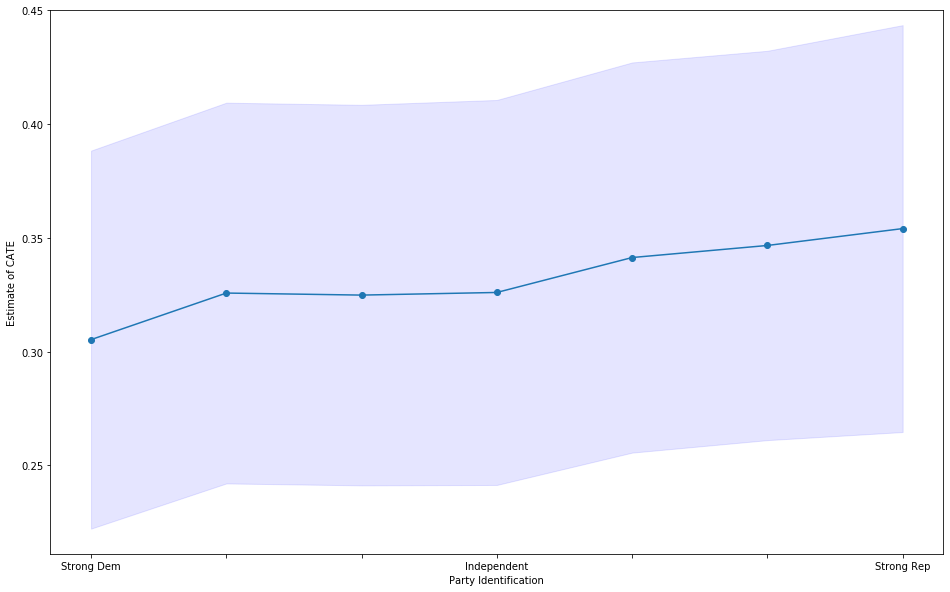
\includegraphics[width = \linewidth]{Graphs/s1_partyid.png}
	\end{subfigure}
	\begin{subfigure} [h] {0.45\linewidth}
		\caption{\textbf{Political Views}}
   	 	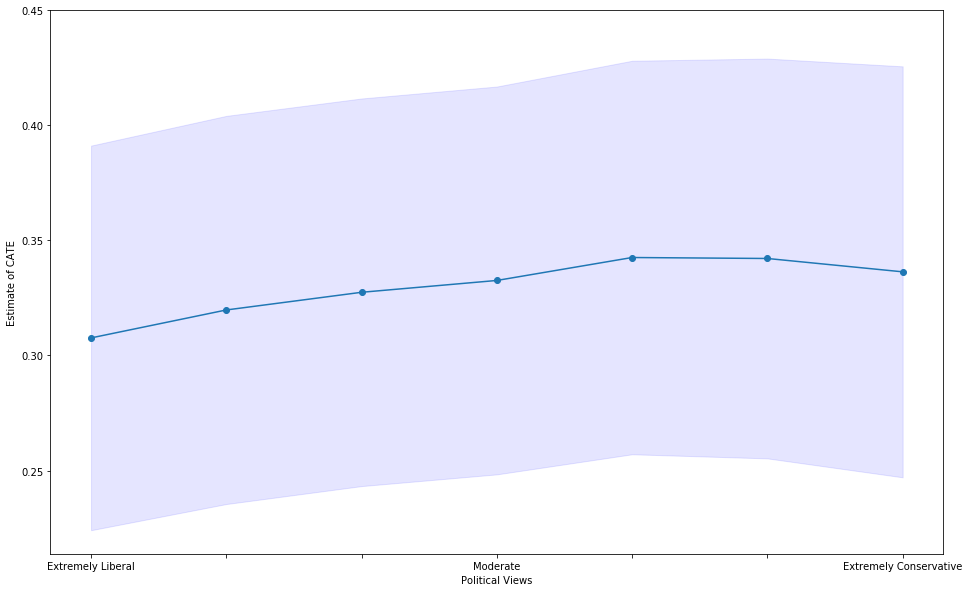
\includegraphics[width = \linewidth]{Graphs/s1_polyview.png}
	\end{subfigure}}
\resizebox*{\textwidth}{!}{
	\begin{subfigure} [h] {0.45\linewidth}
	\caption{\textbf{Age }}
   	 	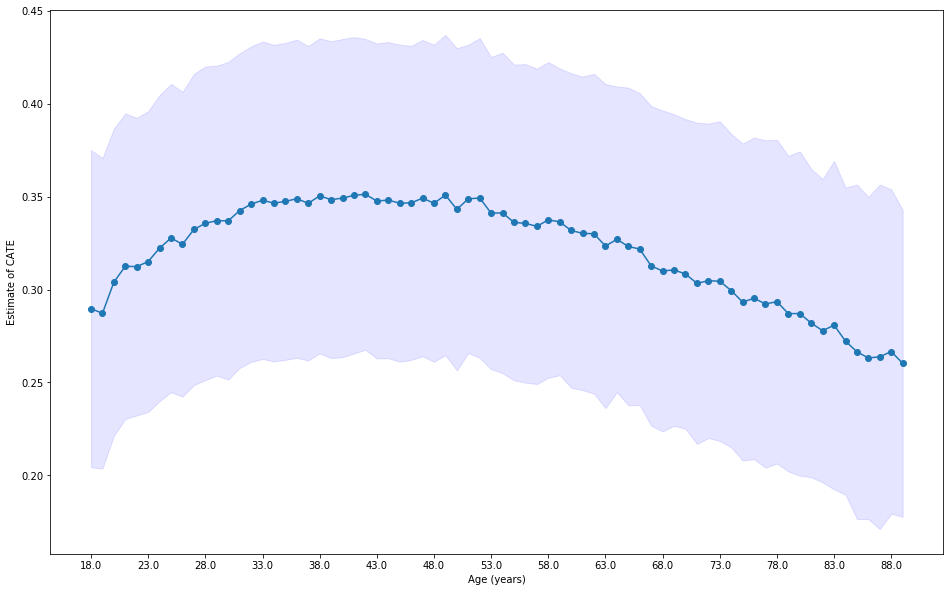
\includegraphics[width = \linewidth]{Graphs/s1_age.png}
	\end{subfigure}
	\begin{subfigure} [h] {0.45\linewidth}
		\caption{\textbf{Education Received}}
   	 	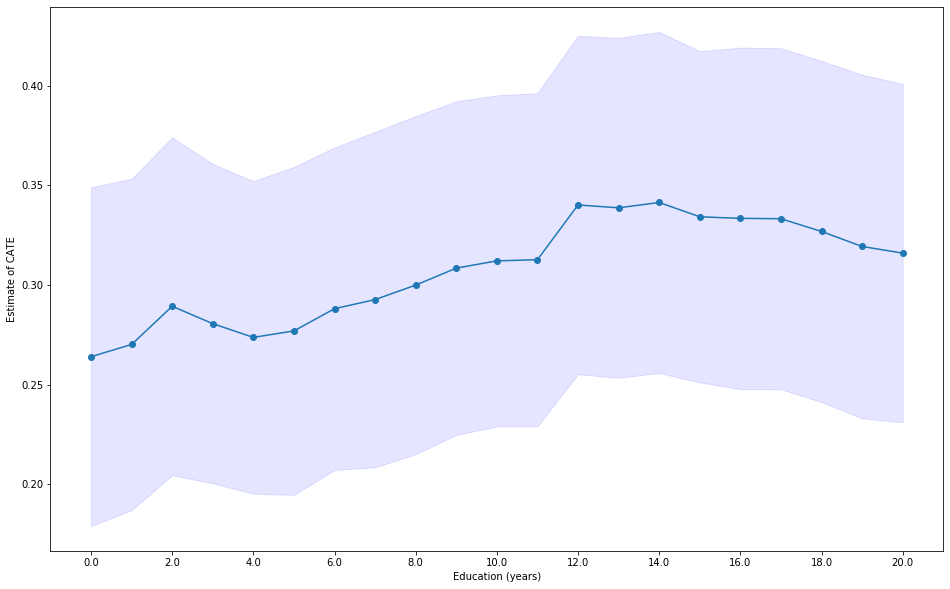
\includegraphics[width = \linewidth]{Graphs/s1_educ.png}
	\end{subfigure}}
\resizebox*{\textwidth}{!}{
	\begin{subfigure} [h] {0.45\linewidth}
	\caption{\textbf{Attitude Toward Blacks}}
   	 	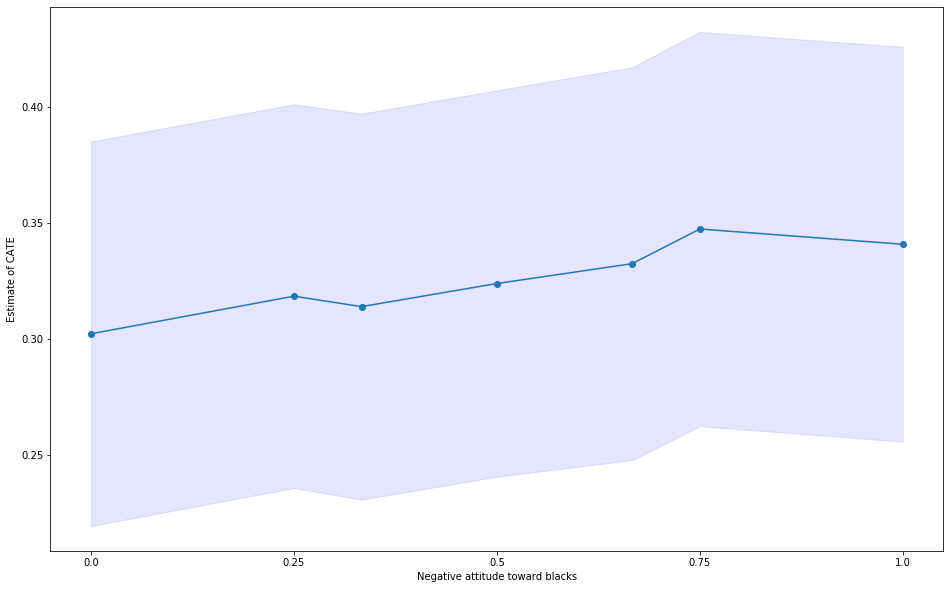
\includegraphics[width = \linewidth]{Graphs/s1_attblack.png}
	\end{subfigure}
	\begin{subfigure} [h] {0.45\linewidth}
		\caption{\textbf{Survey Year}}
   	 	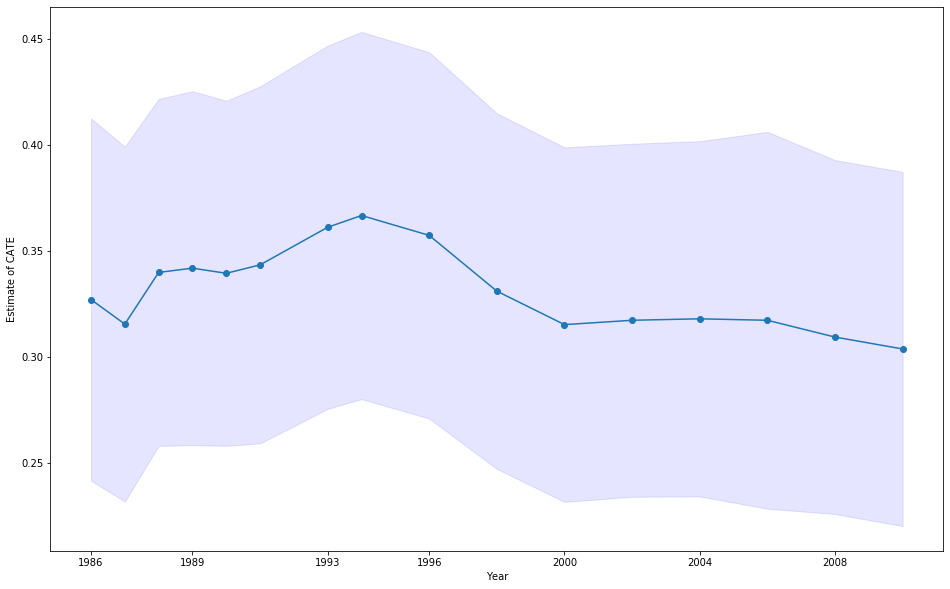
\includegraphics[width = \linewidth]{Graphs/s1_year.png}
	\end{subfigure}}
\end{figure} 

\begin{figure}[h]
\caption{Histogram of CATE Estimates}
	\centering
   	 	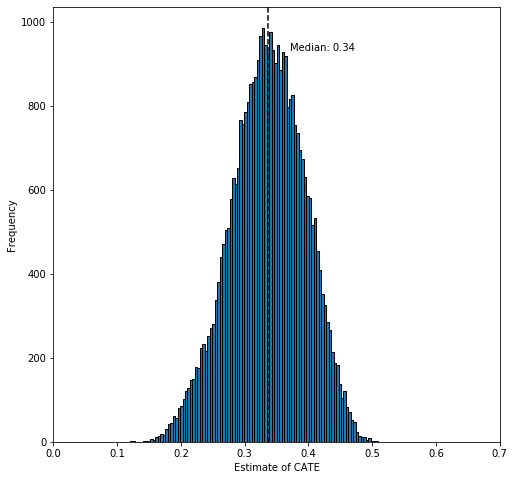
\includegraphics[width = 0.6\linewidth]{Graphs/s1_catefreq.png}
\end{figure} 


\end{document}



















